\section{Illustration}
\label{sec:app}

% when talking about BCN mention
% https://www.researchgate.net/publication/254457523_Urban_form_and_compactness_of_morphological_homogeneous_districts_in_Barcelona_towards_an_automatic_classification_of_similar_built-up_structures_in_the_city#

% all technical details in to an appendix tables from excel should go to notebooks

% spatial signature is a conceptual framework which can materialise in different ways
The classification of built form into spatial signatures is a conceptual framework and
as such, can materialise in different ways depending on the particular implementation of
a description of both form and function and the method of aggregation of enclosed cells
into singatures.
% here we present it applied to five cases from around the world
Here we present the concept applied to five case studies, reflecting different
environments and heterogeneous input data requiring the adaptation of the classification
to individual situations.
% the sample comes with geographical variation - 1, 2, 3, 4, 5
The sample offers a geographical variation covering Europe (Barcelona, Spain), North
America (Houston, TX, United States), South America (Medellin, Colombia), Africa (Dar es
Salaam, Tanzania) and South-east Asia (Singapore),
% that brings different culture, development, planning paradigm, historical and social
% contexts
coupled with cultural diversity, different planning paradigms involved in shaping the
respective environments as well as varied historical and social contexts in which the
selected cities were built (Figure \ref{fig:world_map}).
% at the same time, it brings different input data, varied in both quality and richness
At the same time, the selection brings a variety of input data covering both extremes in
terms of quality (e.g., official mapping in Barcelona vs remote sensing in Houston), the
richness of information on functional aspects of places (e.g., detailed data on the
municipal level in Medellin vs global gridded datasets in Dar es Salaam) and scale
(82,375 units in Barcelona vs 2,043,581 units in Houston).
% we present this variety to illustrate the application and flexibility of the concept
We present this variety to illustrate the flexibility of spatial signatures to
accommodate varied inputs and adapt to a local specificity, while retaining the merit of
the concept.

\begin{figure}
    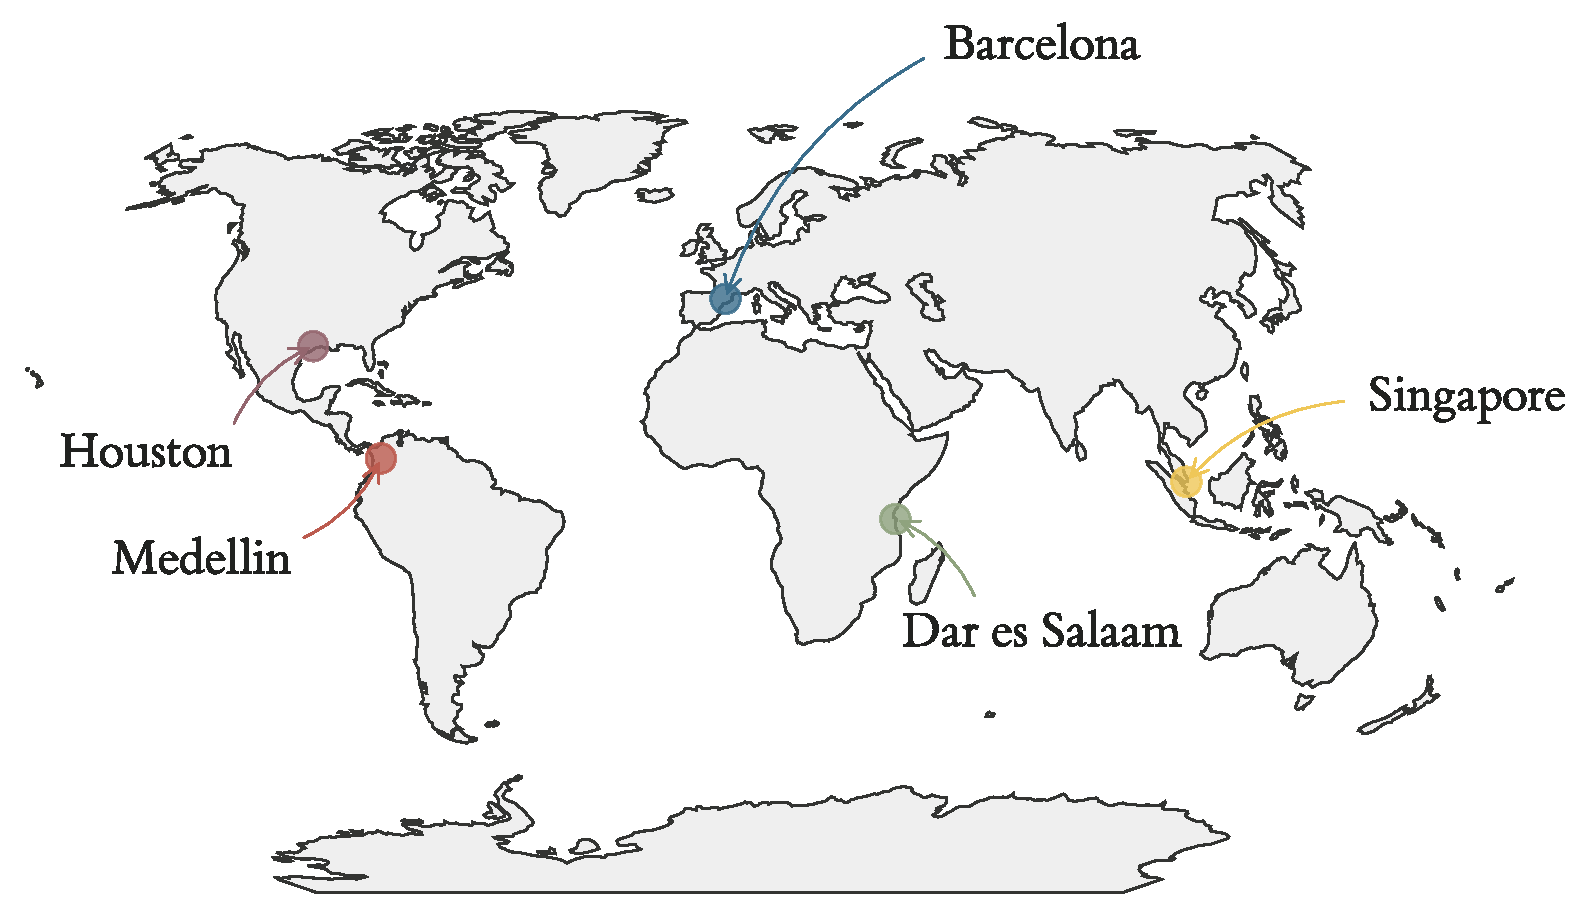
\includegraphics[width=0.75\linewidth, center]{figures/examples_map.pdf}
    \caption{Selection of case studies covering geographical variation,
    cultural diversity, different planning paradigms involved in shaping the
    respective environments as well as varied historical and social contexts in which the
    selected cities were built.}
    \label{fig:world_map}
\end{figure}

\subsection{Method}
%%%%%%%%%%%% Structure 4.1 (squeeze it in a page) introduction of cases - 1 per
% continent; geographical variation, take different cities, cultures, historical moments

%% method - top level outline of the method. Data, Form + convolution, Function,
% Clustering One para on how to build the data - F+F+Convolution, how it varies across
% examples (link to App.)

%%% shall we add conceptual diagram of the method?

% 1. data retrieval from open sources
The delineation of spatial signatures starts with the input data reflecting form and
function of each place. We use enclosed tessellation, outlined in the
\hyperref[sec:ssec:ss_et]{section 3.2}, as a basic spatial unit. Therefore, the input
data should consist of building footprints and physical barriers denoting streets,
railways, and water bodies.
% 2. geographies - enclosures, enclosed tessellation
Using barriers, we first identify the geometry of enclosures to determine the external
boundaries of consequently generated enclosed tessellation.
% 3. characterization of form - primary + convolutions
Resulting set of geometric data is rich enough for a comprehensive morphometric analysis
composed of primary measurable characters, capturing individual aspects of form, and
contextualisation, following the model proposed by
\citealp{fleischmann2021methodological}. In the contextualisation step, we measure the
tendencies of the distribution of each character within the neighbouring context of each
tessellation cell.
% 4. characterisation of function
Function is captured as a heterogeneous set of datasets reflecting aspects from
population to location of points of interest. All aspects are linked to enclosed cells
using the most appropriate method for each data input (e.g., areal interpolation or
network accessibility).\footnote{See \ref{sec:appendix} for details on the
implementation.} The complete list of used characters relfecting both form and function
is available in \ref{sec:appendix}.

% Second para on how we generate signatures (clustering); once we have those we
% dissolve.

% 5. cluster analysis input (all linked to cell)
Spatial signatures are then identified using cluster analysis of tessellation cells
based on their form-function characteristics, combined with the notion of contiguity,
where each contiguous portion of land belonging to a single cluster is seen as a single
signature.
% 6. clustergram
The combined data reflecting both form and function are therefore standardised and
clustered using K-Means clustering. Since the number of classes is not known a priori,
we use clustergram \citep{schonlau2002clustergram} to understand clustering behaviour
within different options and select the optimal number according to its structure.
% 7. clustering
The final clustering is run with 1000 initialisations to ensure the stability of the
results.
% 8. dissolution
The geometry of each spatial signature is then derived as dissolution of a contiguous
patch of enclosed tessellation within the same cluster.


\subsection{Results}
% 4.2 (a page and a half) Results; tell some stories to get reader on board

%%% Para1 how to read the map in an applied way geometries reflect boundaries of spatial
% signatures
Figures \ref{fig:maps1}-\ref{fig:maps2} illustrate the resulting spatial signatures in the respective case
studies.\footnote{For intermediate steps (e.g. clustergram) please refer to
\ref{sec:appendix}.} The geometries reflect the spatial extent of individual signatures
derived from the enclosed tessellation
% colours reflect a type of a signature - two areas within the same type share the
% characteristics; similarity of colours has no meaning
with colour coding reflecting the type of a signature, i.e. the initial cluster. Two
areas within the same type are expected to share the characteristics of built
environment, being more similar (not necessarily the same) to each other than to the
rest of the classes. Note that the similarity of different colours does not encode
similarity of signatures. Also note, that due to varied extent of case studies, maps are
not printed at the same scale.

\begin{figure}
    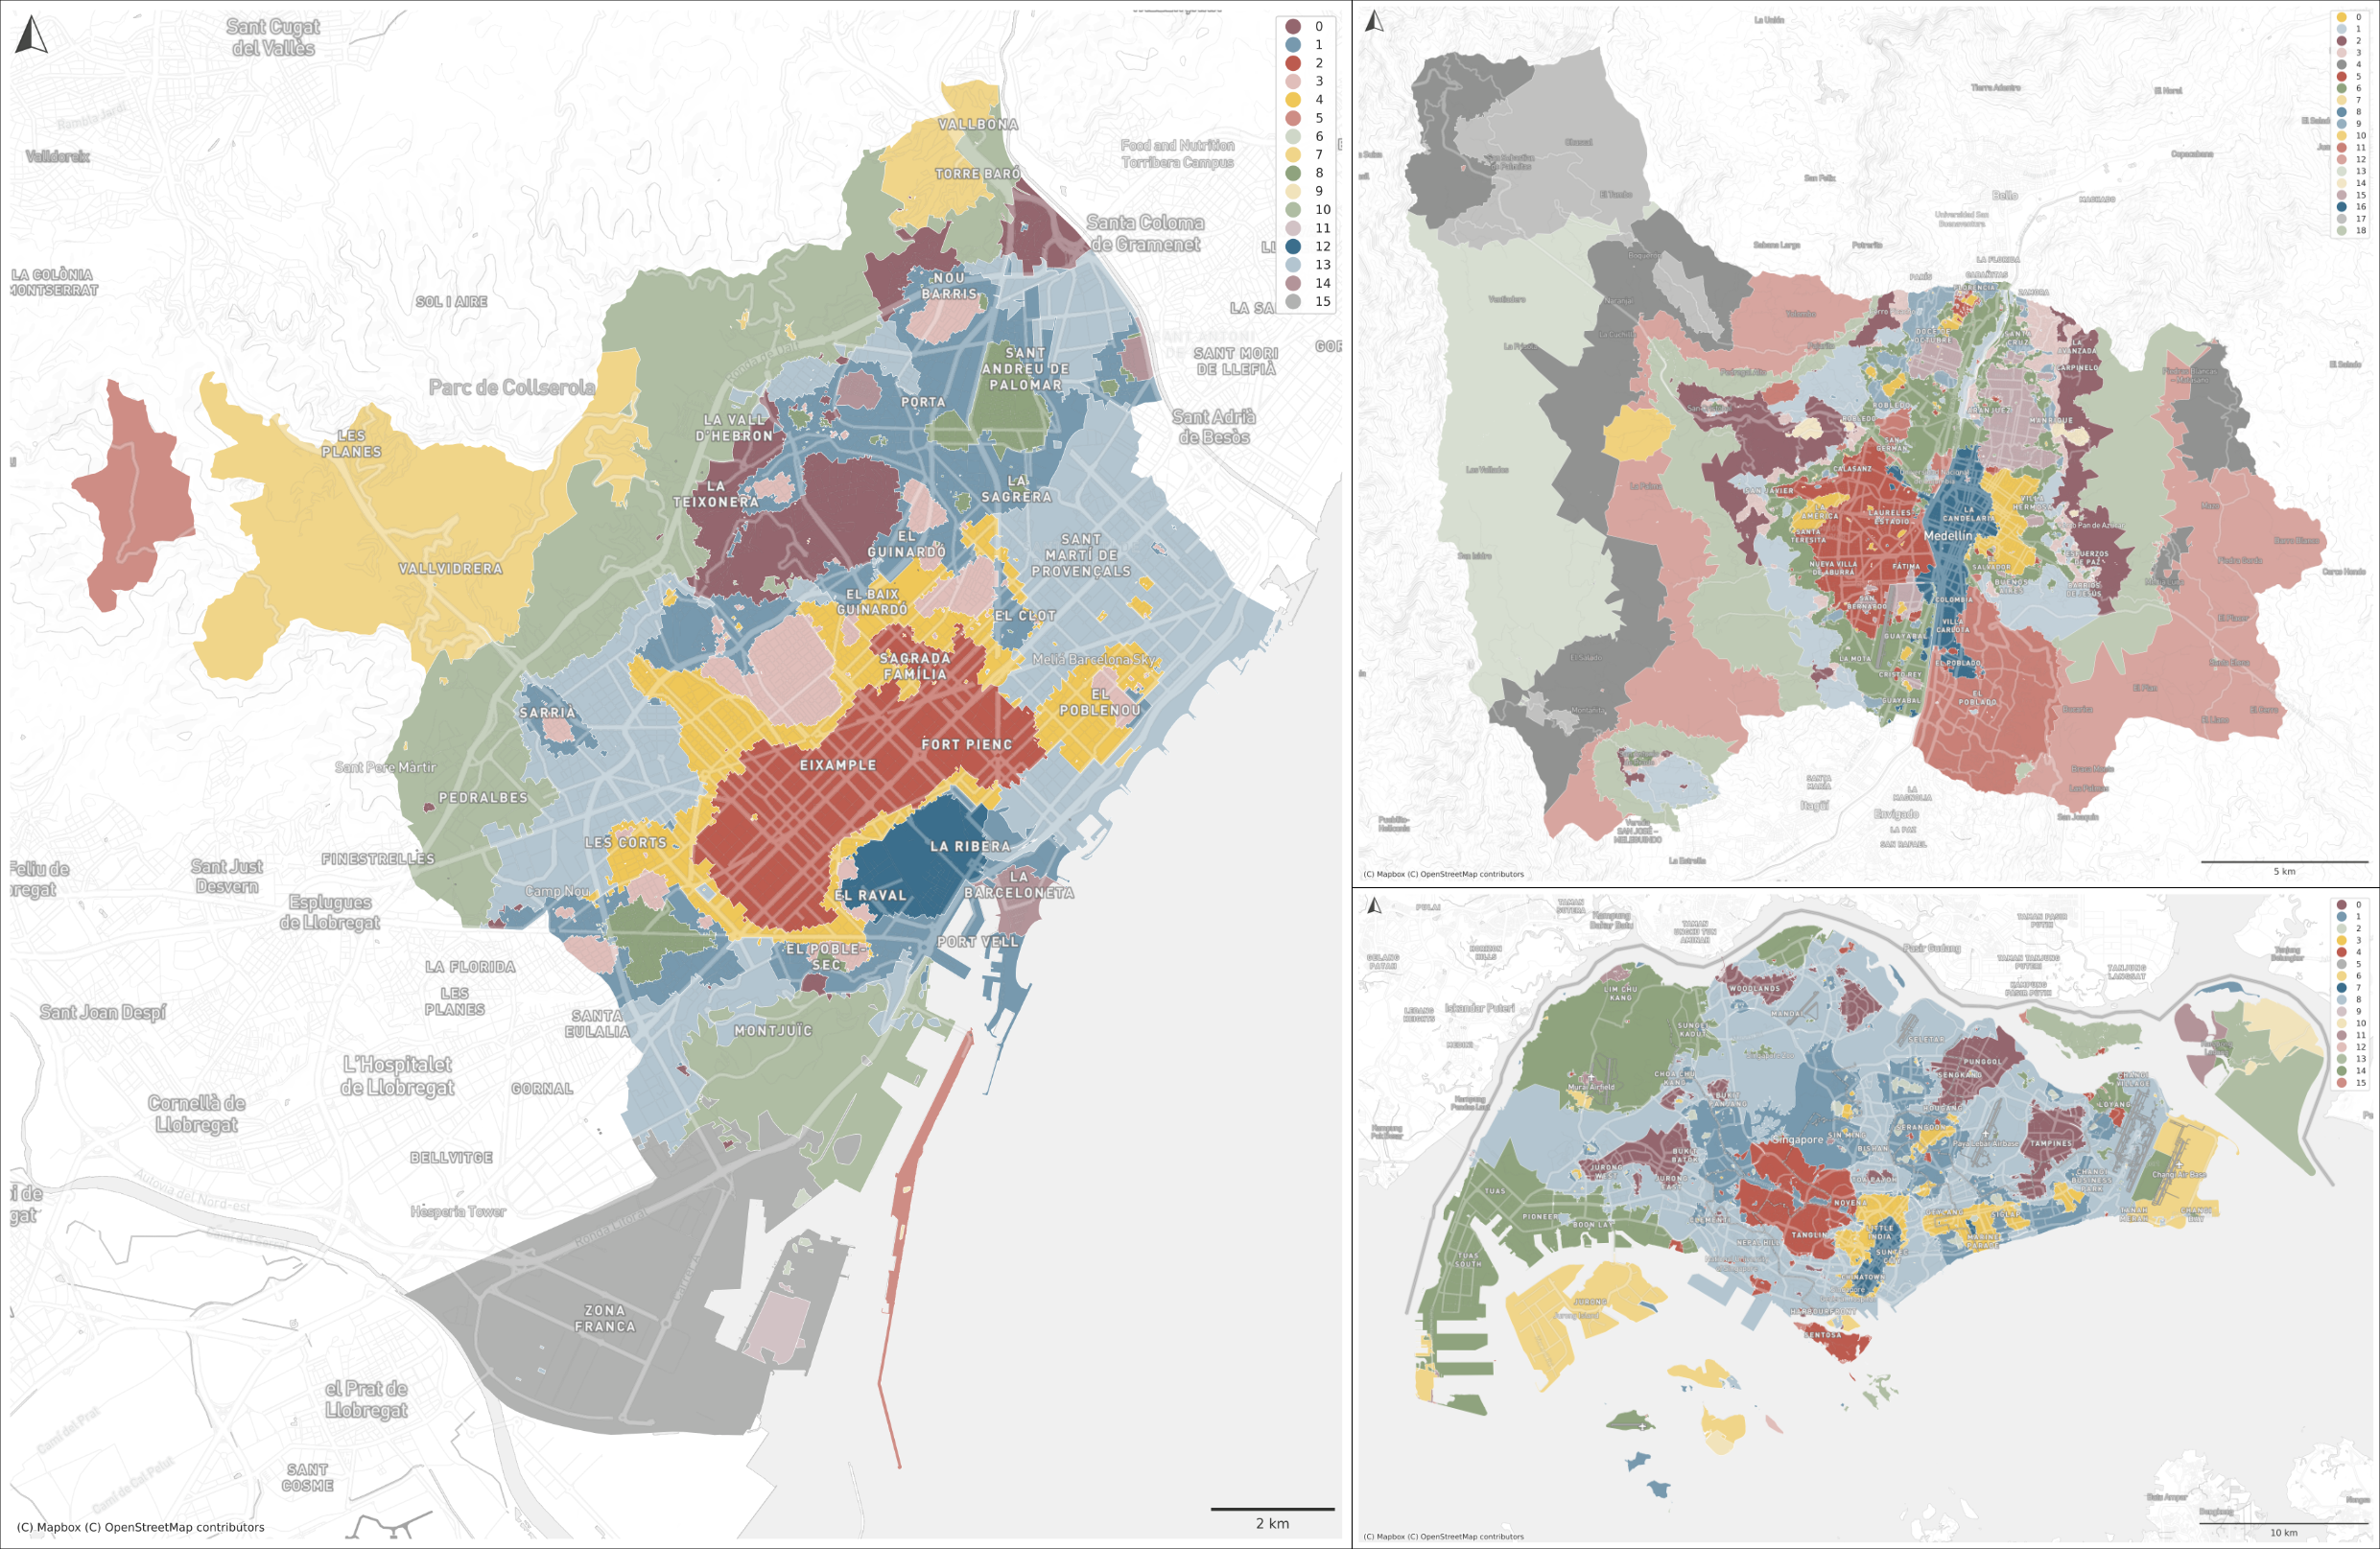
\includegraphics[width=\linewidth]{figures/maps1.png}
    \caption{Resulting Spatial Signatures in the case of Barcelona (A), Singapore (B)
    and Medellin (C). Colours are used to distinguish between types within a single case.}
    \label{fig:maps1}
\end{figure}

%%% Para2 things which are shared/consistent 9-19 clusters, not dependent on the scale
% but reflecting the heterogeneity of a place
The granularity of classification ranges from 9 (Houston) to 19 (Medellin) signature
types per case study. However, the actual number is not dependent on the size of each
city but rather on each place's actual heterogeneity, best illustrated on the comparison
of Houston and Barcelona, the largest (2 million cells) and the smallest (80 thousand
cells) case. Houston, representing north American sprawling urban fabric shows a
considerably smaller diversity of spatial patterns (9 types of spatial signatures) than
Barcelona (16 types), reflecting the richness of their respective historical
developments.
% core clusters and outlier clusters - the abundance varies a lot
The distribution of cluster sizes follows the same pattern of unequal abundance across
all cases. The most extensive types contain between 15 and 28% of all
observations, and the abundance is gradually decreasing towards a small number of
outlier clusters containing less than a per cent of all observations within each sample.
% transition from core to countryside - singapore is exception, its island nature
% restricts such behaviour
All the cases clearly defined both extremes on the urbanisation axis, with delineated
central districts on the one hand and non-urban countryside signatures on the other. The
transition between the two tends to follow the gradual pattern of signatures each less
urban than the previous. The only exception where this tendency is not so profound (but
still present) is Singapore, which geographical extent limited to the defined area of
the main island does not allow the full transition.

%%% Para3 interesting stories from cases (BCN village centres, DeS slums) BCN reflects
% its historical origin - pre-industrial core and village centes, later filled by
% eixample, which has its homogenous core and areas blending into the existing fabric
Barcelona is known for its industrial grid, which is captured as a unique signature.
However, the Cerda’s grid is historically an infill between the city's medieval core and
smaller existing settlements around. Both core and former independent villages are
reflected in the typology of signatures, which reflect the historical origin of distinct
places. The transition between the two, the historical organic fabrics and rigid
Eixample is reflected as another signature, stitching together different patterns into a
coherent city.
% Medellin's change of the pattern as we go up the hill from the central valley
% - central plateu allows more rigid planning reflected in several classes, hillsides
%   are becoming more vernacular
Spatial distribution of signatures in Medellin tells the story of its intricate
topography, even though the input data do not contain any information on altitude. The
city lies in the valley surrounded by steep slopes. While the central parts lie on the
relatively flat floor allowing paradigmatic planning and rigidness of the built
environment, hillsides are becoming more vernacular leading to a sharp urban edge where
the topography does not allow further development.

\begin{figure}
    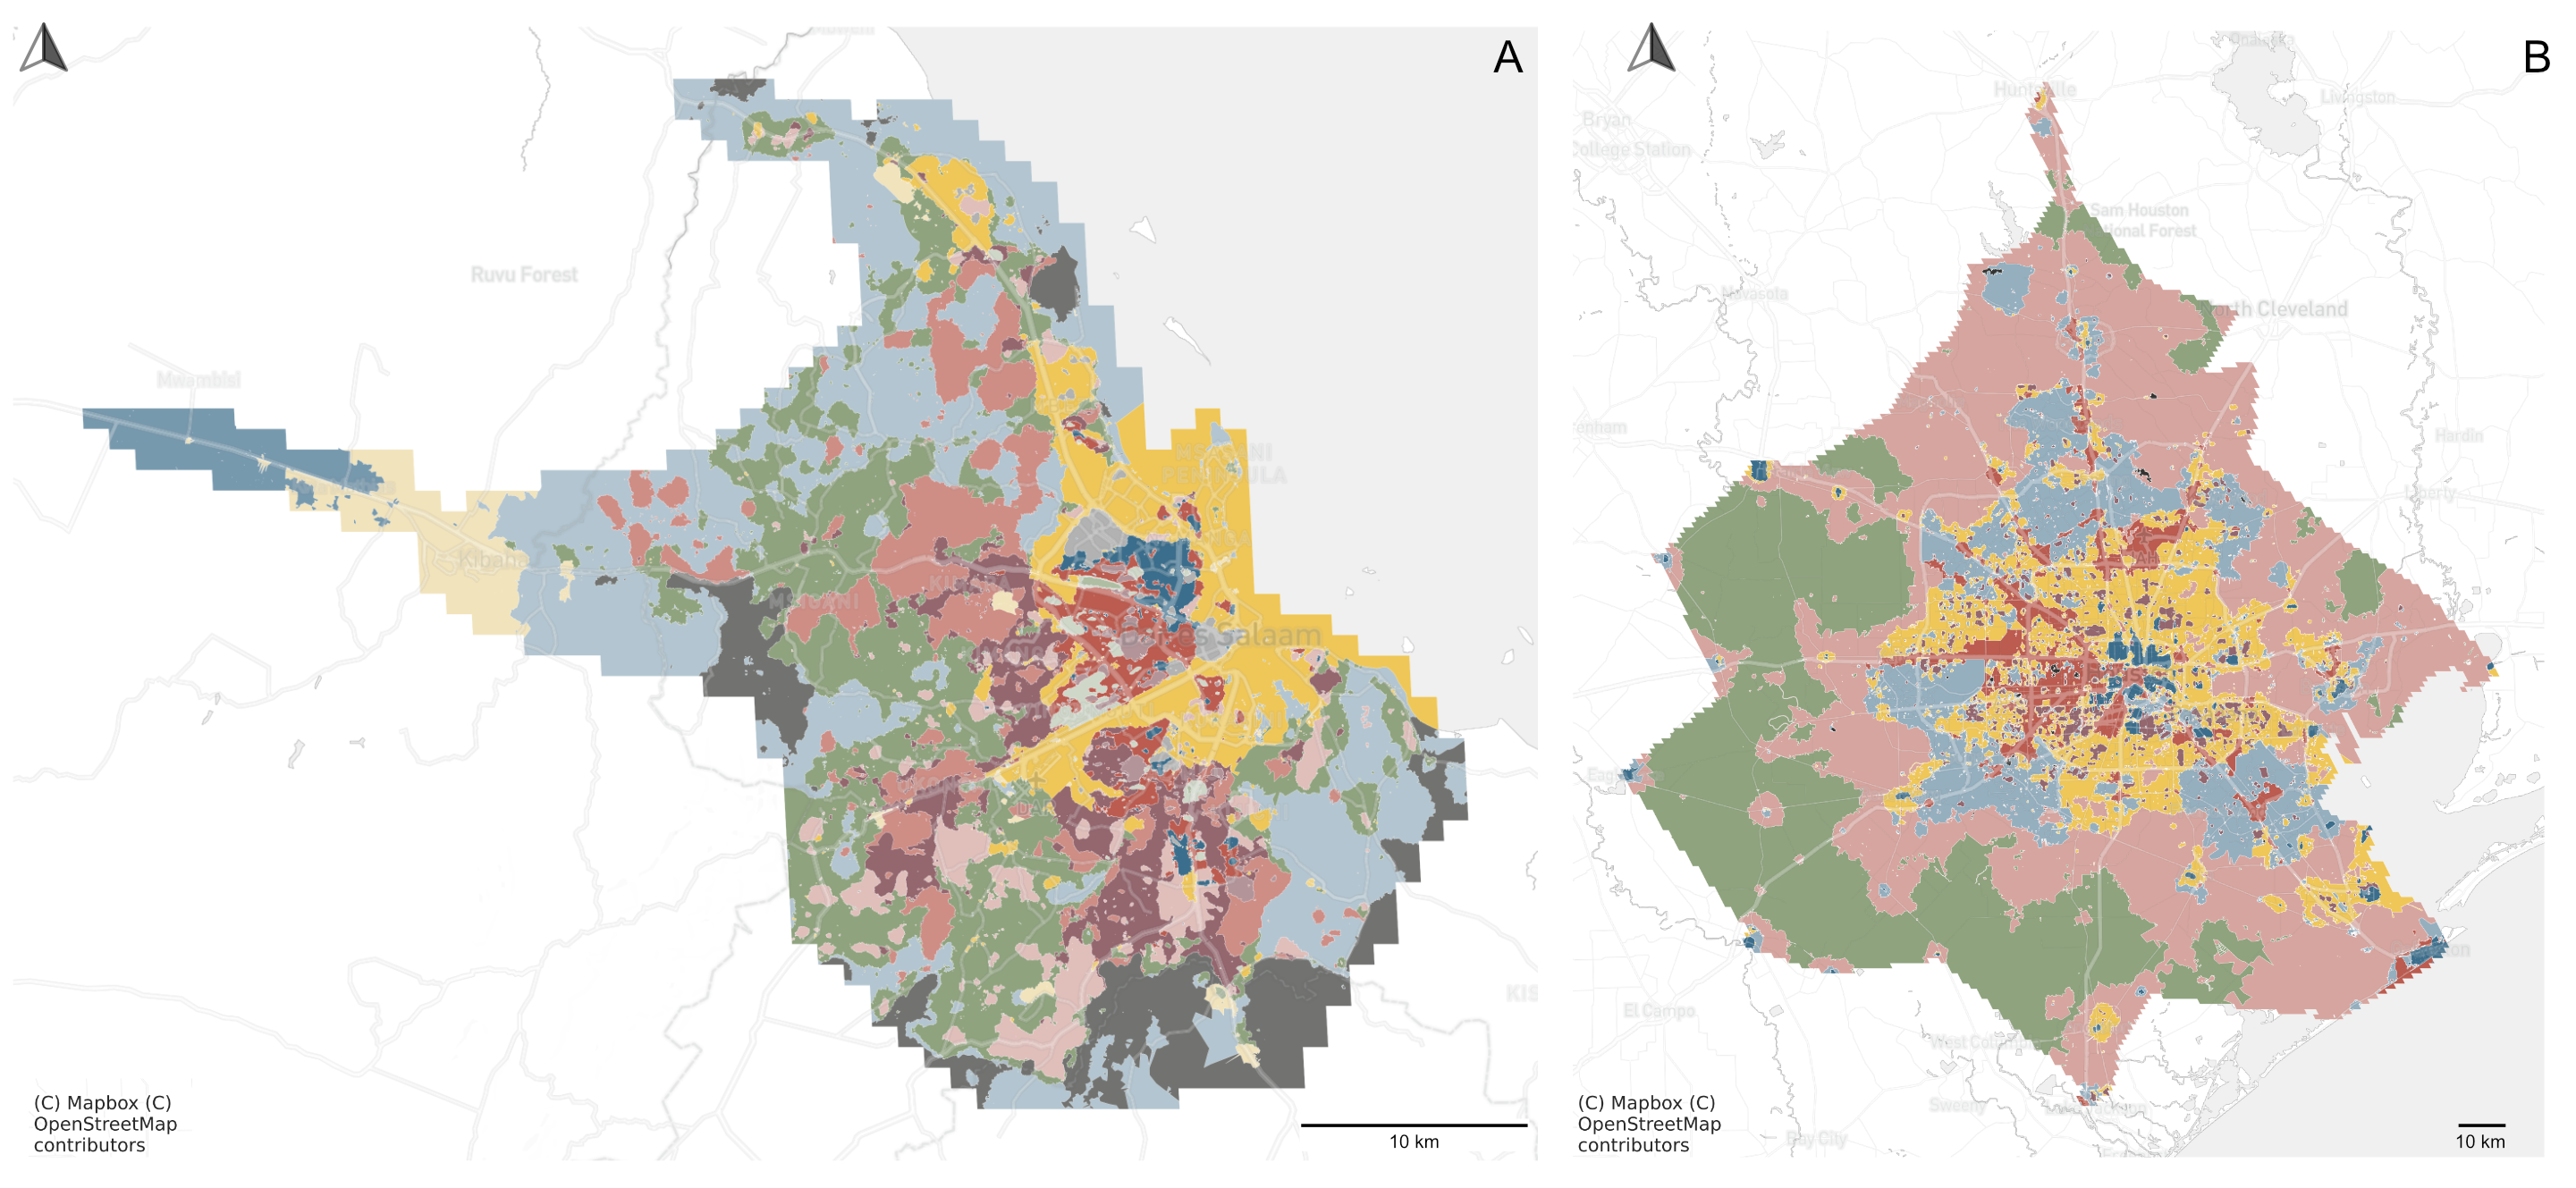
\includegraphics[width=\linewidth]{figures/maps2.png}
    \caption{Resulting Spatial Signatures in the case of Dar es Salaam (A) and Houston (B).
    Colours are used to distinguish between types within a single case.}
    \label{fig:maps2}
\end{figure}

% Dar es Salaam signatures capture different levels of formality, planned, semi-formal
% to informal
Signatures in Dar es Salaam reflect the changes in the formality of development, with
formal areas distributed in the central parts of the city in the vicinity of a
coastline. The transition between different degrees of formality is not always gradual
as the most informal parts of the city are infills of the space not occupied by more
planned neighbourhoods.

% houston and its homogenous sprawl, changing its nature of sprawlness along the time
% and growth, with major roads forming spines of non-residential development
The character of spatial signatures in Houston follows two primary principles. One type
forms the spine of activity spreading from the city centre radially to the suburbs. The
other, filling the areas in between the former, is a story of the deterioration of
compact, walkable urban block into convoluted dendritic street network patterns of
modern suburbs. The change in these predominantly residential signatures is gradual and
reflect the waves of development of the city as it was growing over the years.
% NOTE: Houston signatures are not able to distinguish CBD from the rest of the "spine",
% shall we dicuss that at some point?

% Singapore singature tell the story of its growth. we can follow individual clusters
% and link their origin to different time periods
A similar situation is in Singapore, where different types of signatures can be linked
to the period of the origin of the development of each specific neighbourhood. Contrary
to previous cases, the development and, consequently, spatial signatures followed radial
manner, not entirely contiguous, with major infills built in the last 50 years.
